\documentclass[]{beamer}
\usepackage[english]{babel}
\usepackage[utf8x]{inputenc}
\usepackage{lmodern}
\usepackage[right]{eurosym}
\usepackage{pgfpages}
\usepackage{color}
\usepackage{xcolor}
\usepackage{pgfplotstable}
\usepackage{pgfplots}
\pgfplotsset{width=13cm,compat=1.9}
\definecolor{DARKGREEN}{RGB}{0,100,0}
\usepackage{listings}
\colorlet{mygray}{black!30}
\colorlet{mygreen}{green!60!blue}
\colorlet{mymauve}{red!60!blue}
\colorlet{myyellow}{yellow!50!black}


\lstnewenvironment{C++}{
\lstset{
  backgroundcolor=\color{gray!10},  
  basicstyle=\ttfamily,
  columns=fullflexible,
  breakatwhitespace=false,      
  breaklines=true,                
  captionpos=b,
  belowskip=-2.5em,                    
  commentstyle=\color{DARKGREEN}, 
  extendedchars=true,              
  frame=single,                   
  keepspaces=true,
  showstringspaces=false,             
  keywordstyle=\color{blue},      
  language=c++,                 
  numbers=left,                
  numbersep=5pt,                   
  numberstyle=\tiny\color{blue}, 
  rulecolor=\color{mygray},        
  showspaces=false,               
  showtabs=false,                 
  stepnumber=1,                  
  stringstyle=\color{mymauve},    
  tabsize=3,                      
  title=\lstname                
}}
{}

\lstdefinelanguage{VHDL}{
   morekeywords={
     library,use,all,entity,is,port,in,out,architecture,of,
     begin
   },
   morecomment=[l]--,
   morestring=*[d]{"}
}

\lstnewenvironment{VHI}{
\lstset{
  backgroundcolor=\color{gray!10},  
  basicstyle=\ttfamily,
  columns=fullflexible,
  breakatwhitespace=false,      
  breaklines=true,                
  captionpos=b,
  belowskip=-2.5em,    
  language=VHDL,                 
  commentstyle=\color{DARKGREEN}, 
  extendedchars=true,          
  frame=single,
  showstringspaces=false,                   
  keepspaces=true,
  keywords=[2]{or, and, resize,not,(, ), :, ;},
  keywords=[3]{macro,next, end,else, if, elsif, true, then, is, property, at, t, t_end, false, reset_sequence, assume, prove, freeze, during,[,],t+1,t+2},  
  keywords=[4]{boolean, unsigned, type},          
  keywordstyle=[2]\color{mymauve}, 
  keywordstyle=[3]\color{blue},
  keywordstyle=[4]\color{mygreen},  
  numbers=left,               
  numbersep=5pt,                   
  numberstyle=\tiny\color{blue}, 
  rulecolor=\color{mygray},        
  showspaces=false,               
  showtabs=false,                 
  stepnumber=1,                  
  stringstyle=\color{mymauve},    
  tabsize=3,                      
  title=\lstname                
}}
{}


\usetheme{Frankfurt}

%\beamertemplatenavigationsymbolsempty
%\setbeameroption{show notes on second screen=left}


\title{Multilevel Hardware Generation and Verification}
\subtitle{Presentation of master thesis}
\author{Harald Øvsthus}
 \setbeamertemplate{navigation symbols}
{  \insertslidenavigationsymbol 
\insertframenavigationsymbol   
\insertsubsectionnavigationsymbol  
  \insertsectionnavigationsymbol
  \insertdocnavigationsymbol  
  \insertbackfindforwardnavigationsymbol 
 \hspace{1em}  
\usebeamerfont{footline} 
   \insertframenumber/\inserttotalframenumber }
 \setcounter{page}{1} 
\pagenumbering{arabic} 
\begin{document}
	\begin{frame}[plain]
\addtocounter{framenumber}{-1}
		\titlepage
	\end{frame}

	\begin{frame}
\addtocounter{framenumber}{-1}
		\frametitle{Contents of presentation}
		\tableofcontents
	\end{frame}

	\section{Introduction}
	\begin{frame}
		\frametitle{Introduction}
	          \onslide<1->{\textbf{Idea:}}
                  \begin{itemize}
	           \item<1->Generate AMBA-AHB systems at the ESL and RTL
                   \item<1->Generate properties from the ESL, automatically refine them
                  \end{itemize}
                  \onslide<2->{\textbf{Goals:}}
                    \begin{enumerate}
                      \item<2-> Abstraction
                      \item<2-> Soundness
                    \end{enumerate}     
	\end{frame}

\section{Generator}
 \begin{frame}
  \frametitle{Generator}
   \begin{center}
   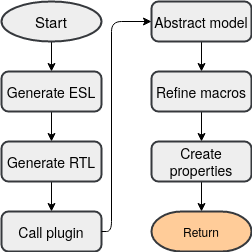
\includegraphics[scale=0.5]{pics/Gen_flow.png}
   \end{center}
 \end{frame}

    
       \section{ESL overview}
         \begin{frame}
          \frametitle{ESL overview}
             \begin{center}
             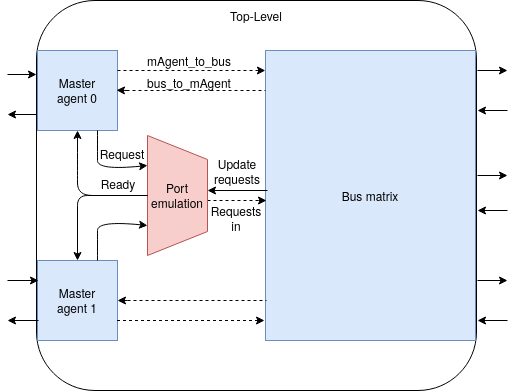
\includegraphics[scale=0.5]{pics/syslev_new.png}
             \end{center}
         \end{frame}

      
         \begin{frame}
          \frametitle{ESL overview continued}
          \begin{center}
          \only<1>{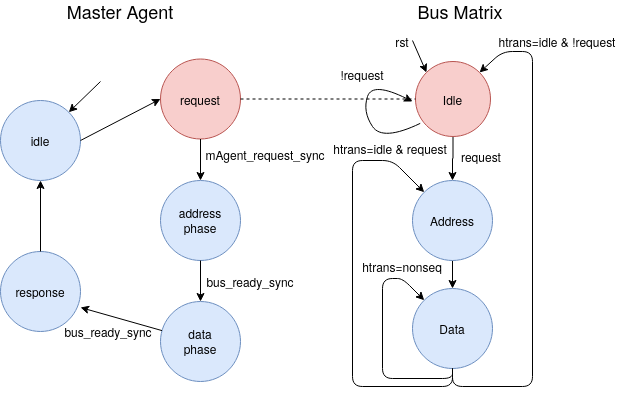
\includegraphics[scale=0.4]{pics/agent_bus_fsm0.png}}
          \only<2>{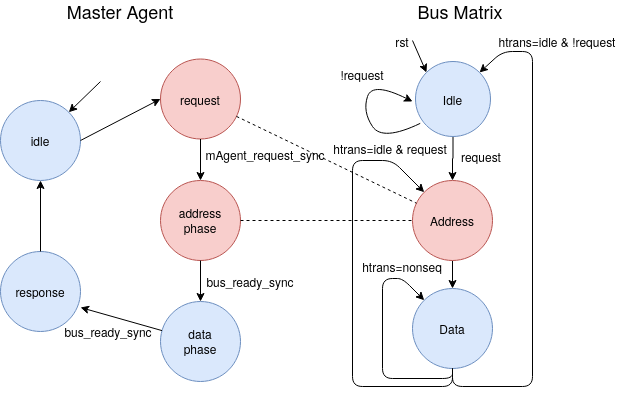
\includegraphics[scale=0.4]{pics/agent_bus_fsm1.png}}
          \only<3>{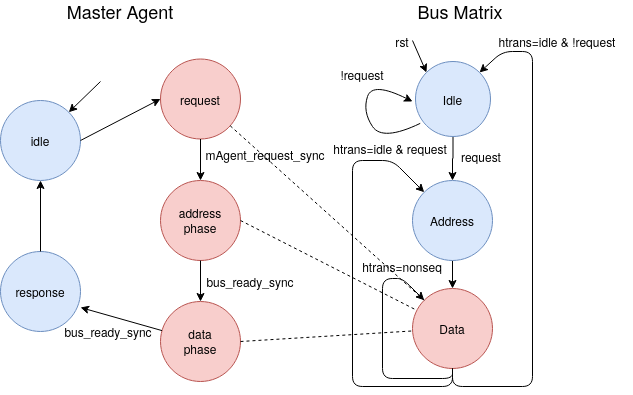
\includegraphics[scale=0.4]{pics/agent_bus_fsm2.png}}
          \end{center}
         \end{frame}


\begin{frame}[fragile]
\frametitle{Bus matrix; data state}
\begin{C++}
if(state == data)
  if(payload.haddr == slave_range){
    agent_to_bus->get(payload.hwdata);

    bus_to_slave->write(payload):
    slave_to_bus->read(response);

    bus_to_agent->set(response);

   }else{
     bus_to_agent->set(error);
     }

//Handle requests, end data phase
\end{C++}
\end{frame}
 

         \begin{frame}[fragile]
           \frametitle{Emulated port, reason}
            \begin{C++}
if(mAgent_request0->peek()) //requesting
else if(mAgent_request1->peek())  
else if(mAgent_request2->peek())  

if(bus_ready0->peek())
if(bus_ready1->peek()) //waiting
if(bus_ready2->peek()) //waiting
            \end{C++}

         \end{frame}

         \begin{frame}[fragile]
           \frametitle{Emulated port, internal}
            \begin{C++}
update_requests->read() //wait for sync

if(mAgent_request0->peek()) 
  try_read(); //unblock
else if(mAgent_request1->peek()) 
  try_read();  
else if(mAgent_request2->peek())  
  try_read();

requests_out->set(requests); //forward requests

if(bus_ready0->peek()) try_read();
if(bus_ready1->peek()) try_read(); //unblock
if(bus_ready2->peek()) try_read(); //unblock
            \end{C++}

         \end{frame}

         \begin{frame}[fragile]
           \frametitle{Emulated port, bus matrix}
            \begin{C++}
//Bus matrix data state

update_requests->try_write();
requests_in->get(requests);

if(requests.master0){
//get payload
}else if(requests.master1){

            \end{C++}

         \end{frame}






\section{RTL overview}
         \begin{frame}
           \frametitle{RTL overview}
           \begin{columns}
            \column{0.5\textwidth}
             \begin{itemize}
             \item<1-> Reuse open source AHB architecture
             \item<2-> Agents implement the protocol
             \end{itemize}
            \column{0.5\textwidth}
             \centering
             \only<1>{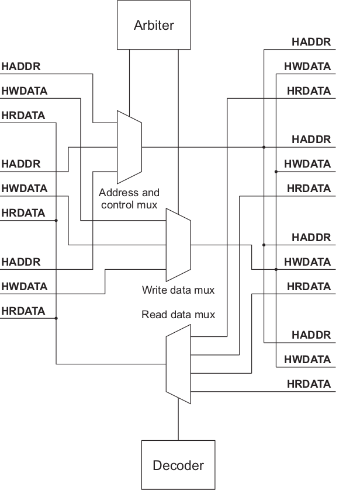
\includegraphics[width=0.7\textwidth]{pics/OS_HW.png}}
             \only<2>{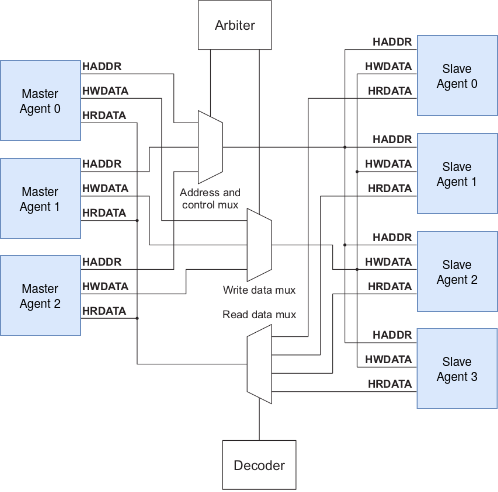
\includegraphics[width=\textwidth]{pics/RTL_overview.png}}
           \end{columns}
         \end{frame}


       \section{Completeness}
       \begin{frame}
        \frametitle{Completeness}
          \begin{enumerate}
              \item<1-> All I/O listed in completeness description
              \item<1-> All completeness checks hold, no constraints
          \end{enumerate}
       \end{frame}

       \begin{frame}
         \frametitle{Completeness continued}
           \begin{center}
           \only<1>{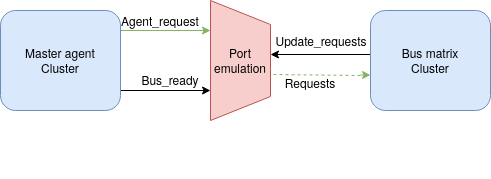
\includegraphics[width=\textwidth]{pics/port_refine0.png}}
           \only<2>{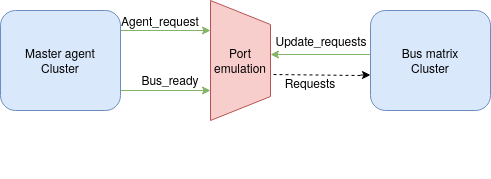
\includegraphics[width=\textwidth]{pics/port_refine1.png}}
           \end{center}

       \end{frame}
       \begin{frame}[fragile]
         \frametitle{Completeness continued}
       \begin{VHI}
macro Agent_request_notify := hbusreq0 end macro;
 

macro Requests_sig_m0_request := hbusreq0 end macro;
macro Requests_sig_m1_request := hbusreq1 end macro;
       \end{VHI}
       \end{frame}

       \begin{frame}[fragile]
         \frametitle{Completeness continued}
       \begin{VHI}
macro Agent_request_sync := hgrant0 and hready0 end

macro Bus_ready_sync := hready0 end macro;



Update_requests_notify :=
hready0 and hready1 or
hgrant0 and hready0 or
hgrant1 and hready1
end macro;

       \end{VHI}
       \end{frame}
  

       \section{Simulation}

         \begin{frame}
           \frametitle{Simulation}
            \begin{center}
            \only<1>{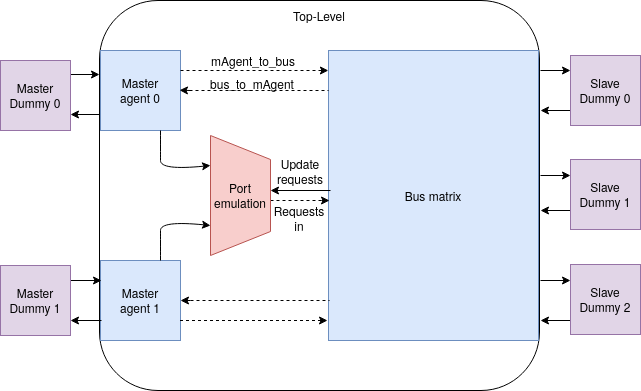
\includegraphics[scale=0.5]{pics/tb_esl.png}}
            \only<2>{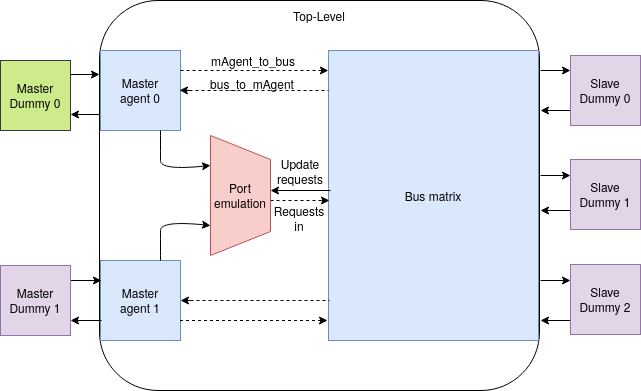
\includegraphics[scale=0.5]{pics/tb_esl1.png}}
            \only<3>{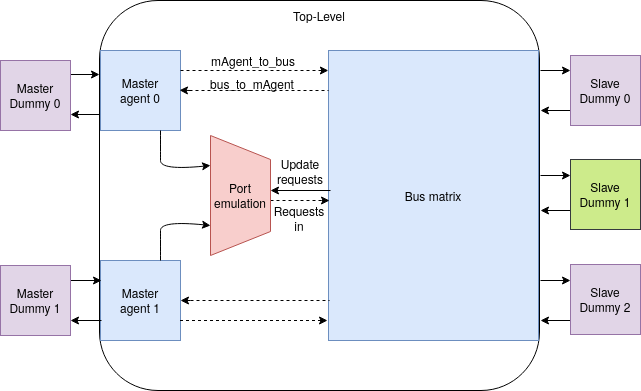
\includegraphics[scale=0.5]{pics/tb_esl2.png}}
            \only<4>{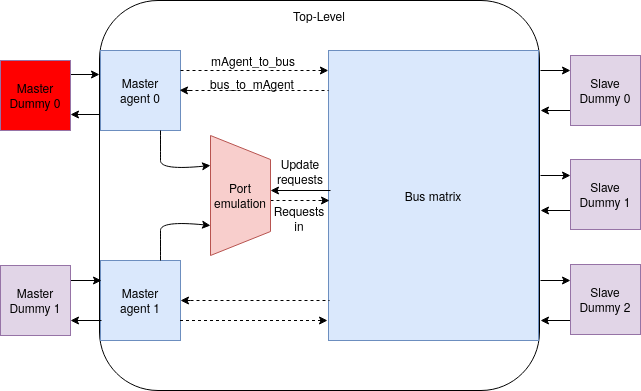
\includegraphics[scale=0.5]{pics/tb_esl3.png}}
            \end{center}
         \end{frame}

        \section{Results}

\begin{frame}
\frametitle{Resource comparison}
\begin{table}[hbt] 
  \begin{tabular}{ l r r r r r}
  \hline 
  \hline
      & \multicolumn{2}{c}{\textbf{\_\_\_\_\_\_}RTL\textbf{\_\_\_\_\_\_}} & \multicolumn{3}{c}{\textbf{\_\_\_\_\_\_\_\_\_\_}PPA\textbf{\_\_\_\_\_\_\_\_\_\_}} \\
   & inp./out. & FFs & inp./out & var. & states \\
    \hline
  AHB & - & 114 & - & 5 & 3 \\
  
  Per slave & 107/114 & 193 & 1/1 & - & 2 \\
 
  Per master & 107/114 & 286 & 2/4 & 12 & 5 \\
    \hline
    \hline  
  \end{tabular}
\caption{AHB system component comparison}
\label{tab:stats}
\end{table}
\end{frame}

         \begin{frame}
\frametitle{Simulation Time Comparison}
\begin{center}
\begin{tikzpicture}[scale=0.5]
\begin{axis}[
    ybar,
    enlargelimits=0.15,
    legend style={at={(0.5, -0.15)},
      anchor=north,legend columns=-1},
    ylabel={T sec},
    symbolic x coords={1 slave, 5 slaves, 10 slaves, 15 slaves},
    xtick=data,
    nodes near coords,
    nodes near coords align={vertical},
]
\only<1>{\addplot coordinates { (1 slave,261)(5 slaves,266)(10 slaves,270)(15 slaves,284) };}
 

\only<1>{\addplot coordinates {(1 slave,161)(5 slaves,166)(10 slaves,180)(15 slaves,195)};}

\only<1>{\addplot coordinates {(1 slave,77)(5 slaves,86)(10 slaves,103)(15 slaves,125)};}
    
\only<1->{\addplot coordinates {(1 slave,7)(5 slaves,7)(10 slaves,7)(15 slaves,7)};}
\only<1>{\legend{RTL 1 master  , RTL 2 masters  , RTL 3 masters  , ESL all sizes}}


\end{axis}
\end{tikzpicture}
\end{center}
\end{frame}

\begin{frame}
\frametitle{Properties and Proof times}
 \begin{columns}
\column{0.5\textwidth}
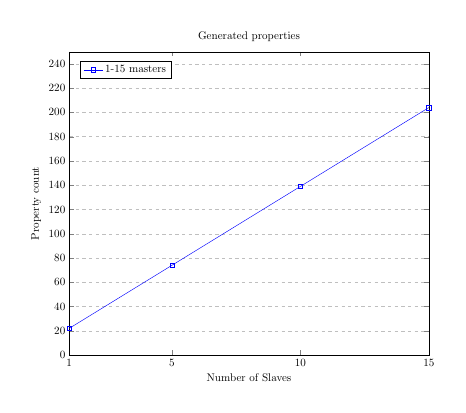
\begin{tikzpicture}[scale=0.4]
\begin{axis}[
    title={Generated properties},
    xlabel={Number of Slaves},
    ylabel={Property count},
    xmin=1, xmax=15,
    ymin=0, ymax=250,
    xtick={1,5,10,15},
    ytick={0,20,40,60,80,100,120,140, 160, 180, 200, 220, 240},
    legend pos=north west,
    ymajorgrids=true,
    grid style=dashed,
]
\addplot[
    color=blue,
    mark=square,
    ]
    coordinates {
    (1,22)(5,74)(10,139)(15,204)

    };
    \addlegendentry{1-15 masters}


\end{axis}
\end{tikzpicture}
\column{0.5\textwidth}
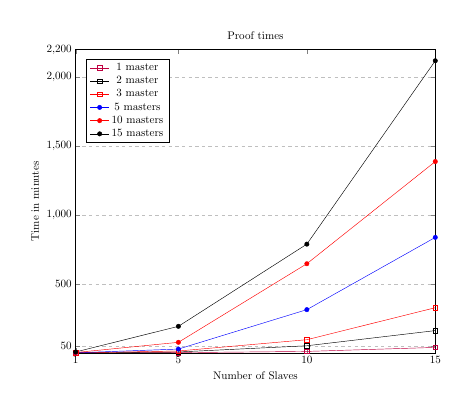
\begin{tikzpicture}[scale=0.4]
\begin{axis}[
    title={Proof times},
    xlabel={Number of Slaves},
    ylabel={Time in minutes},
    xmin=1, xmax=15,
    ymin=0, ymax=2200,
    xtick={1,5,10,15},
    ytick={50,500, 1000, 1500, 2000, 2200},
    legend pos=north west,
    ymajorgrids=true,
    grid style=dashed,
]
\addplot[
    color=purple,
    mark=square,
    ]
    coordinates {
    (1,1)(5,2)(10,11)(15,40)

    };
    \addlegendentry{1 master}

\addplot[
    color=black,
    mark=square,
    ]
    coordinates {
    (1,1)(5,7)(10,52)(15,162)

    };
    \addlegendentry{2 master}

\addplot[
    color=red,
    mark=square,
    ]
    coordinates {
    (1,1)(5,14)(10,96)(15,328)

    };
    \addlegendentry{3 master}

\addplot[
    color=blue,
    mark=*,
    ]
    coordinates {
   (1,1)(5,28)(10,314)(15,838)
    };
    \addlegendentry{5 masters}

\addplot[
    color=red,
    mark=*,
    ]
    coordinates {
    (1,3)(5,77)(10,647)(15,1388)
    };
    \addlegendentry{10 masters}

\addplot[
    color=black,
    mark=*,
    ]
    coordinates {
    (1,7)(5,193)(10,789)(15,2119)
    };
    \addlegendentry{15 masters}
    
\end{axis}
\end{tikzpicture}

 \end{columns}
\end{frame}


\subsection{Starvation}
 \begin{frame}
  \frametitle{Starvation}
        \begin{center}
        \only<1>{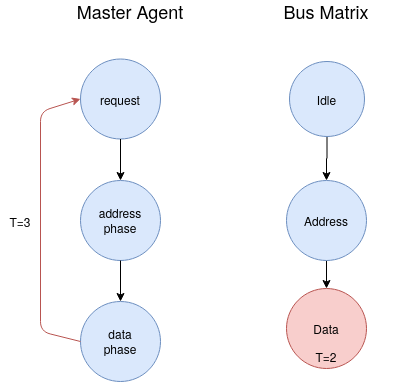
\includegraphics[scale=0.5]{pics/Starvation0.png}}
        \only<2>{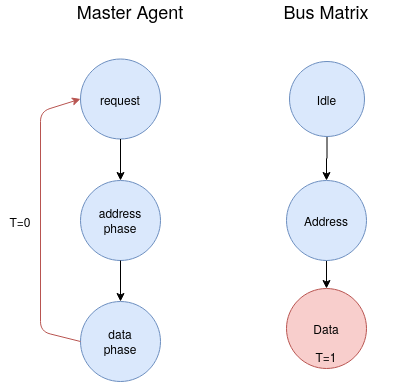
\includegraphics[scale=0.5]{pics/Starvation1.png}}
        \only<3>{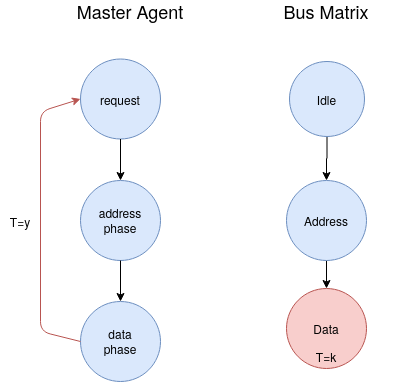
\includegraphics[scale=0.5]{pics/Starvation2.png}}
        \end{center}
 \end{frame}



         \begin{frame}
           \frametitle{Starvation comparison}
          \begin{columns}
             \column{0.5\textwidth}
\begin{tikzpicture}[scale=0.4]
\begin{axis}[
    title={Starvation, RTL},
    xlabel={Master granted},
    ylabel={Clock delay},
    xmin=1, xmax=15,
    ymin=0, ymax=60,
    xtick={1,2,3,4,5,6,7,8,9,10,11,12,13,14,15},
    ytick={0,2,4,6,8,10,12,14,16,18,20,22,24,26,28,30,32,34,36,38,40,42,44,46,48,50,52,54,56,58,60},
    legend pos=north west,
    ymajorgrids=true,
    grid style=dashed,
]
\only<1,2->{\addplot[
    color=blue,
    mark=square,
    ]
    coordinates {
    (1,0)(2,0)(3,0)(4,0)(5,2)(6,4)(7,6)(8,8)(9,10)(10,12)(11,14)(12,16)(13,18)(14,20)(15,22)

    };
    \addlegendentry{Out of range}}

\only<2->{\addplot[
    color=purple,
    mark=square,
    ]
    coordinates {
    (1,0)(3,0)(5,6)(7,14)(9,22)(11,30)(13,38)(15,46)

    };
    \addlegendentry{write success}}

\only<2->{\addplot[
    color=red,
    mark=*,
    ]
    coordinates {
    (1,0)(2,0)(4,2)(6,10)(8,18)(10,26)(12,34)(14,42)(15,46)

    };
    \addlegendentry{read error}}

\only<2->{\addplot[
    color=black,
    mark=square,
    ]
    coordinates {
    (1,0)(2,0)(3,0)(4,1)(5,4)(6,7)(7,10)(8,13)(9,16)(10,19)(11,22)(12,25)(13,28)(14,31)(15,34)
    };
    \addlegendentry{read success}}

\only<2->{\addplot[
    color=gray,
    mark=square,
    ]
    coordinates {
    (1,0)(2,0)(3,0)(4,3)(5,8)(6,13)(7,18)(8,23)(9,28)(10,33)(11,38)(12,43)(13,48)(14,53)(15,58)

    };
    \addlegendentry{write error}}

\end{axis}
\end{tikzpicture}
             \column{0.5\textwidth}
\begin{tikzpicture}[scale=0.4]
\begin{axis}[
    title={Starvation, ESL},
    xlabel={Master granted},
    ylabel={Wait time},
    xmin=1, xmax=15,
    ymin=0, ymax=25,
    xtick={1,2,3,4,5,6,7,8,9,10,11,12,13,14,15},
    ytick={0,2,4,6,8,10,12,14,16,18,20,22,24},
    legend pos=north west,
    ymajorgrids=true,
    grid style=dashed,
]

\only<3->{\addplot[
   color=red,
    mark=square,
    ]
    coordinates {
    (1,0)(2,0)(3,0)(4,2)(5,3)(6,4)(7,5)(8,6)(9,7)(10,9)(11,11)(12,13)(13,14)(14,21)(15,22)

    };
    \addlegendentry{in range, wait(rand()\%y+1, SC\_PS), $z=4$}}

\only<3->{\addplot[
   color=blue,
    mark=square,
    ]
    coordinates {
    (1,0)(2,0)(3,0)(4,2)(5,3)(6,4)(7,5)(8,6)(9,7)(10,8)(11,9)(12,11)(13,12)(14,14)(15,16)

    };
    \addlegendentry{in range, wait(rand()\%y+1, SC\_PS), $z=2$}}



\only<2->{\addplot[
   color=purple,
    mark=*,
    ]
    coordinates {
    (1,0)(2,0)(3,0)(4,2)(5,3)(7,5)(8,6)(10,8)(12,10)(14,12)(15,13)

    };
    \addlegendentry{in range, wait(y, SC\_PS)}}


\only<1->{\addplot[ 
  color=black,
    mark=square,
    ]
    coordinates {
    (1,0)(2,0)(3,0)(4,1)(5,3)(6,4)(7,5)(9,7)(11,9)(13,11)(15,13)

    };
    \addlegendentry{out of range, wait(y, SC\_PS)}}

%\only<2,5>{\addplot[ 
%  color=red,
%    mark=*,
%    ]
%    coordinates {
%    (1,0)(2,0)(3,0)(4,2)(5,2)(6,4)(7,4)(8,6)(9,6)(10,8)(11,8)(12,10)(13,10)(14,12)(15,12)
%
%    };
%    \addlegendentry{out of range, y$*$wait(0, SC\_PS)}}


\end{axis}
\end{tikzpicture}
 \end{columns}
 \end{frame}    


\section{Burst transfers}
 \begin{frame}
  \frametitle{Concept: Burst transfers}
         \only<1>{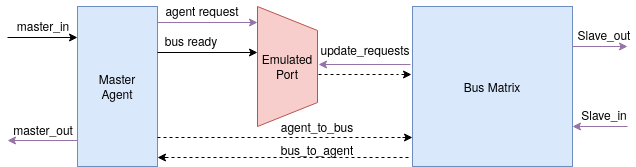
\includegraphics[scale=0.5]{pics/burst_esl_stripped.png}}
         \only<2->{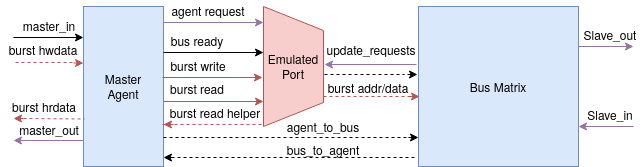
\includegraphics[scale=0.5]{pics/burst_esl.png}}
    \begin{itemize}
      \item<1-> Payloads are extended to include burst
      \item<2-> Additional ports are required 
    \end{itemize}  
 \end{frame}

 \begin{frame}[fragile]
   \frametitle{Bursts continued} 
 

\begin{C++}
if(4-beat incremental){
payload.htrans = seq | seq | seq | idle;
//concatenate control signals

payload.haddr1 = address + 4; //word data size
payload.haddr2 = address + 8;
//haddr 4-15 = 0

payload.hwdata3 = data3;
payload.hwdata4 = 0;
//hwdata 4-15 = 0

shared_out_hwdata = data3; //final values
shared_out_htrans = idle;  
}

\end{C++}

\end{frame}

\begin{frame}[fragile]
 \frametitle{Bursts continued} 
 
\begin{VHI}
macro hwdata4_sig := 
if(16-beat burst) then
prev(hwdata,11)  --align for 16 beats
elsif(8-beat burst) then
prev(hwdata,3)   --align for 8 beats
else
resize(0,32)     --eliminate for 4 beats
end if;
end macro;
\end{VHI}

 \end{frame}

\begin{frame}
 \frametitle{Bursts continued}
 Where do we stand with completeness?
 \begin{itemize}
  \item<1-> Determination requirements
  \item<2-> Duration of transfer
 \end{itemize}
\end{frame}

\section{Outlook}

\begin{frame}
 \frametitle{Outlook}
 Further research:
 \begin{itemize}
  \item<2-> Formally verified emulated port
  \item<3-> Monitor for fixed-priority arbitration
 \end{itemize}
\end{frame}

\subsection{Conclusion}

\begin{frame}
 \frametitle{Conclusion}
 \begin{itemize}
  \item<1-> Generates AHB for single transfers with properties.
  \item<2-> High level of abstraction is achieved
  \item<3-> Burst transfers are shown to be feasible
 \end{itemize}
\end{frame}


\begin{frame}
 Questions?
\end{frame}

\end{document}
